\section{Multispectral Segmentation}
In this section, we show the application of our setup for material segmentation.
We deploy our method using two setups : (1)  Using the full spectrum light source for table top material identification (2) Using our portable setup for scenes in the wild.
In the first setup, due to the bulky sensor setup, we were constraint to table-top environments as discussed in \Sec \ref{sec:fullspectrum}.
Therefore while we exploit the full spectrum capabilities of our approach, we cannot evaluate it with complex scenes.
Therefore, in \Sec \ref{sec:realforest}, we show the material segmentation of branches and leaves in real forest areas of Masoala Rainforest in Zurich Zoo using the $3$ wavelength illumination source used in \cite{ESL}.
We specifically focus on segmenting branches and leaves as applications for this have a great impact in robotics, where for example when navigating in a foliage would be possible by pushing the leaves but not the branches.
% In the case of material differentiation, we use our full spectrum light source setup.
% This allows us to exploit fully the capabilities of our setup.
% Note however that as our setup is bulky, it limits the operation to indoor table-top environments.
% Additionally, the field of view of the light source also limits our evaluations to a small operating area.
% To demonstrate the full capabilities of multispectral imaging for material segmentation, we consider the task of segmenting different parts of a tree namely leaves and branches.
% This is an important task for robotics because \mm{ToDO add christians motivation}.

\subsection{Full spectrum indoor scenes}
\label{sec:fullspectrum}
% \subsection{Multispectral material differentiation}
\begin{figure}[hbt!]
    \centering
    \begin{tikzpicture}
    \node[anchor=south west,inner sep=0] (image) at (0,0) {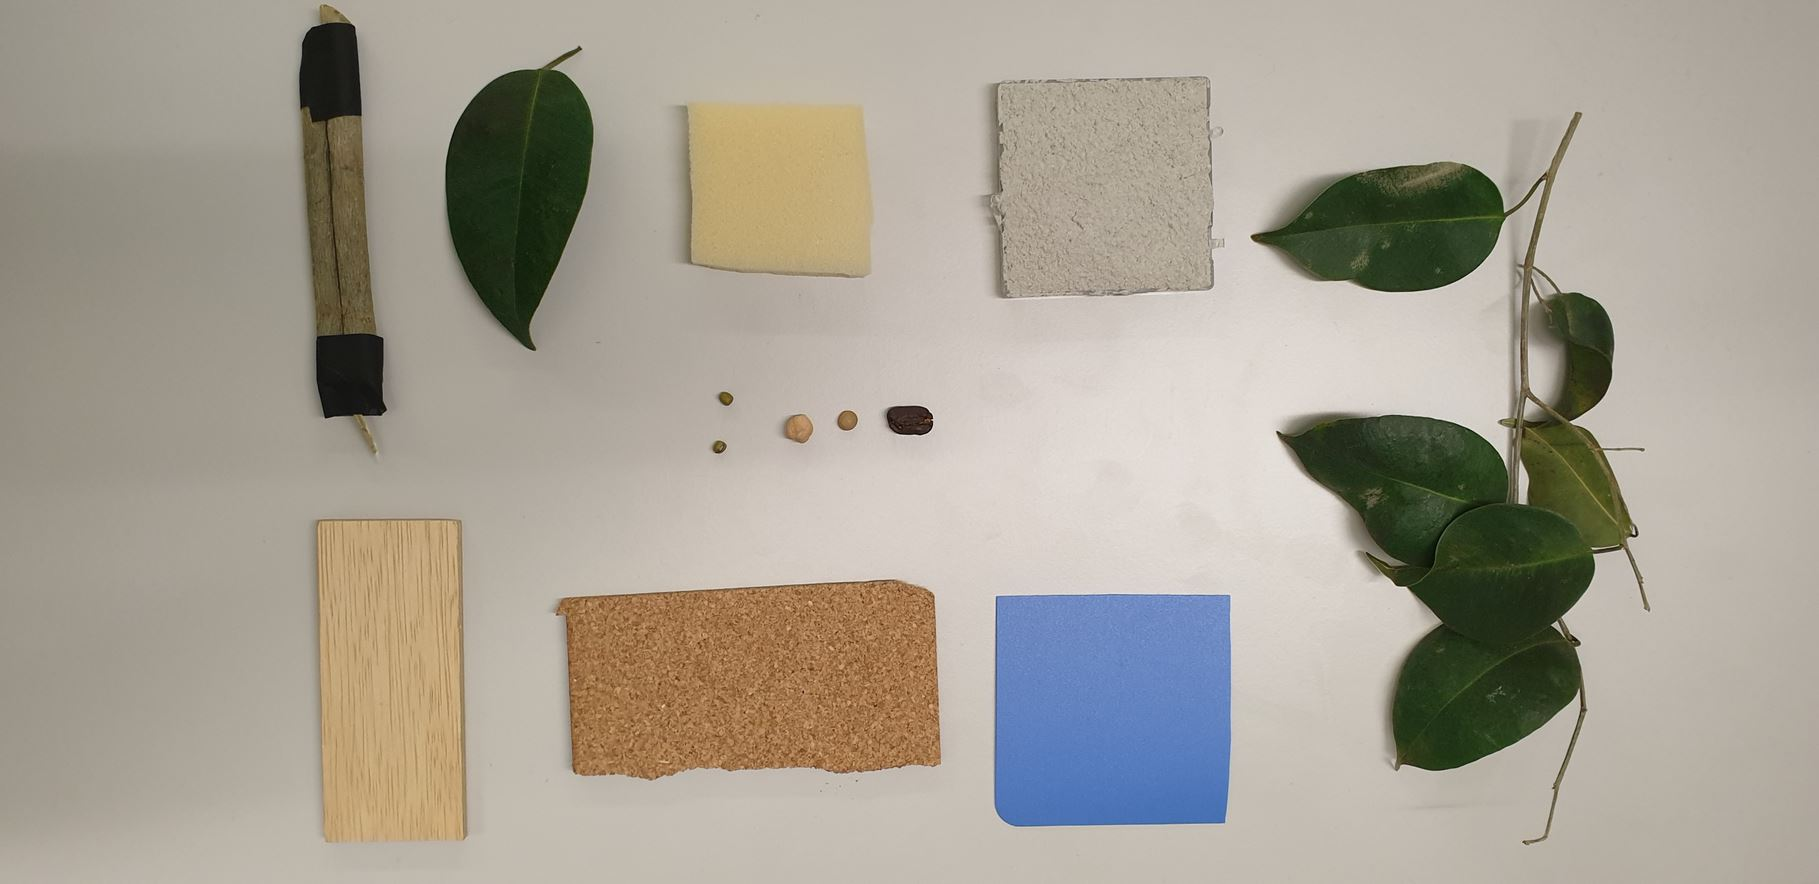
\includegraphics[width=\linewidth]{chapters/papers/ED/resources/images/multi-spectral/material_samples.png}};
    \begin{scope}[x={(image.south east)},y={(image.north west)}]
        \node [rounded corners, fill=white] at (0.18, 0.92) {branch};
        \node [rounded corners, fill=white] at (0.29, 0.92) {leaf};
        \node [rounded corners, fill=white] at (0.42, 0.92) {foam};
        \node [rounded corners, fill=white] at (0.6, 0.92) {plaster};
        \node [rounded corners, fill=white] at (0.21, 0.38) {wood};
        \node [rounded corners, fill=white] at (0.42, 0.38) {cork};
        \node [rounded corners, fill=white] at (0.6, 0.38) {plastic};
    \end{scope}
    \end{tikzpicture}%
\caption{Materials used for evaluating our setup}
\label{fig:materials}
\end{figure}

We evaluate our approach using the full spectrum light source shown in \Fig \ref{fig:generalSetup}.
% We evaluate the performance using material samples such as plastic, wood, foam, plaster, cork, leaf and branch 
We illuminate the material samples, in particular a 99\% reflective reference panel, plastic, wood, foam, plaster, cork, leaf, branch, and various beans and capture the response in the event camera\Fig \ref{fig:materials}.
The same scenes are observed  using a MicaSense RedEdge-MX Dual camera system, which serves as ou baseline.
For all of the samples, the groundtruth is collected using a spectrometer which measures the reflected light.
We plot the RMSE graphs for each sample and compare its accuracy to MicaSense multispectral camera \cite{} in \Fig \ref{fig:materialResponses}.
Qualitatively, the reflectance measured by the event camera follow the groundtruth curves well.
The normalized measurements are quite sensitive to outliers, which causes particularly high errors for the branch in which the reflectance of the last wavelength is far too high.
% While the MicaSense is only sensitive to few wavelengths, our setup can capture a wider wavelength range.
% We also see that response of our method closely aligns with the MicaSense and spectrograph groundtruth.


% \mm{ToDo add graphs}
% \nn{added 3 most accurate graphs}
\begin{figure}
\centering
\imageTable{resources/plots/multi-spectral}{individual-curves}{/}{plastic, leaf, foam}{}{}{2.75}{2.75}
% \imageTable{plots/MSI}{individual_curves}{/}{cork, plaster, plastic, wood}{}{}{3}{3}
\caption{Normalized Material Reflectance Spectra \mm{make these plots better visible}}
\label{fig:materialResponses}
\end{figure}

\subsection{Real forest demonstration}
\label{sec:realforest}
As the full spectrum light source restricts our operation to indoor table-top material samples, we validate our approach for real-world scenes using our \cite{ESL} setup, which has a restricted spectrum of illumination wavelengths.
To quantitatively evaluate our approach, we use a automatic data labelling tool using segment anything model and fine-tuned by humans.
We have $31$ RGB-D scenes divided into $21$ training sequences and $10$ test sequences.
For each pixel, we predict $3$ labels: (1)  leaves, (2) branches and (3) background.
We compare the performance of segmentation using only RGB images, only depth and RGB-D fusion using the intersection-over-union (IoU) score for leaves and branches.
Since leaves are both more present and individually larger in most of the images, their class is generally easier to detect. Inter-class variation is also lower for leaves and many errors are caused by the predictor misclassifies brown or overexposed
leaves as branches. 
Overall, the results suggest that RGB information is more important for the semantic segmentation task than only using depth images. 
The combination of the two, however, depth improves the results by 30\%.
We show qualitative results for the combined approach in \Fig \ref{fig:segment}.

\begin{table}[t]
    \centering
    \begin{tabular}{lrrr}
    \toprule
    channels  & \multicolumn{3}{c}{IoU}\\
     & leaves & branches & mean\\
    \midrule
    depth  & 0.534 & 0.045 & 0.365\\
    RGB  & 0.681 & 0.200 & 0.441\\
    RGBD  & \textbf{0.706} & \textbf{0.288} & \textbf{0.497}\\
    \bottomrule
    \end{tabular}
    \caption{The pipeline is run with only RGB, only depth, and all channels. For each of them, I compare their results with only initial connected component clustering and additional fine spectral clustering.}
    \label{tab:segmentation_results}
\end{table}
\subsection{Semantic segmentation}
Lastly, we also evaluate our setup for segmenting the different parts of trees, namely branches and leaves.
The spectral and depth information can be utilized for semantic segmentation specifically to identify leaves and branches.
\begin{figure*}
    \centering
    \imageTable{resources/images/segmentation}{03,04,05}{/}{depth, rgb, out}{}{depth, rgb, segmentation}{7.3}{4.5}
    \caption{Segmentation results}
    \label{fig:segment}
\end{figure*}
